\chapter{Probleme in der Umsetzung}
In diesen Kapitel möchte ich auf probleme bei der Entwicklung des Prototypes eingen und kurz auf allgemeine Problem beim Arbeiten mit KI-Systeme bei der Entwicklung von Videospielen.

\section{Ablenkung und Abschweifung}
In \ref{chatgpt-ptompt-Midjourney-04} Umsetzung habe ich mir einen Prompt für Midjourne ausgeben lassen für einen Abentuerer mit Fuchskopf. Der Gund warum ich ChatGPT nicht aufgefordert habe mir eine Ausgabe von Martin Luther ausgeben zu lasse, das ich abgelenkt war und mir spontan die Idee von einem Abenteurer mit Fuchskopf gekommen ist.

KI-Systeme geben dn
\section{Einarbeitungszeit}
KI-Systeme benötigen Einarbeitungszeit. Bis ich PIFuHD zum laufen gebracht habe, vergingen Tage mit neuen versuchen. Abildung \ref{erstemalpifuhdblender} zeigt das erste Ergebnis was ich mit der Kombination Midjourney und PIFuHD erzeugt habe.
\begin{figure}
	\centering
	\begin{minipage}[t]{0.45\linewidth}
		\centering
		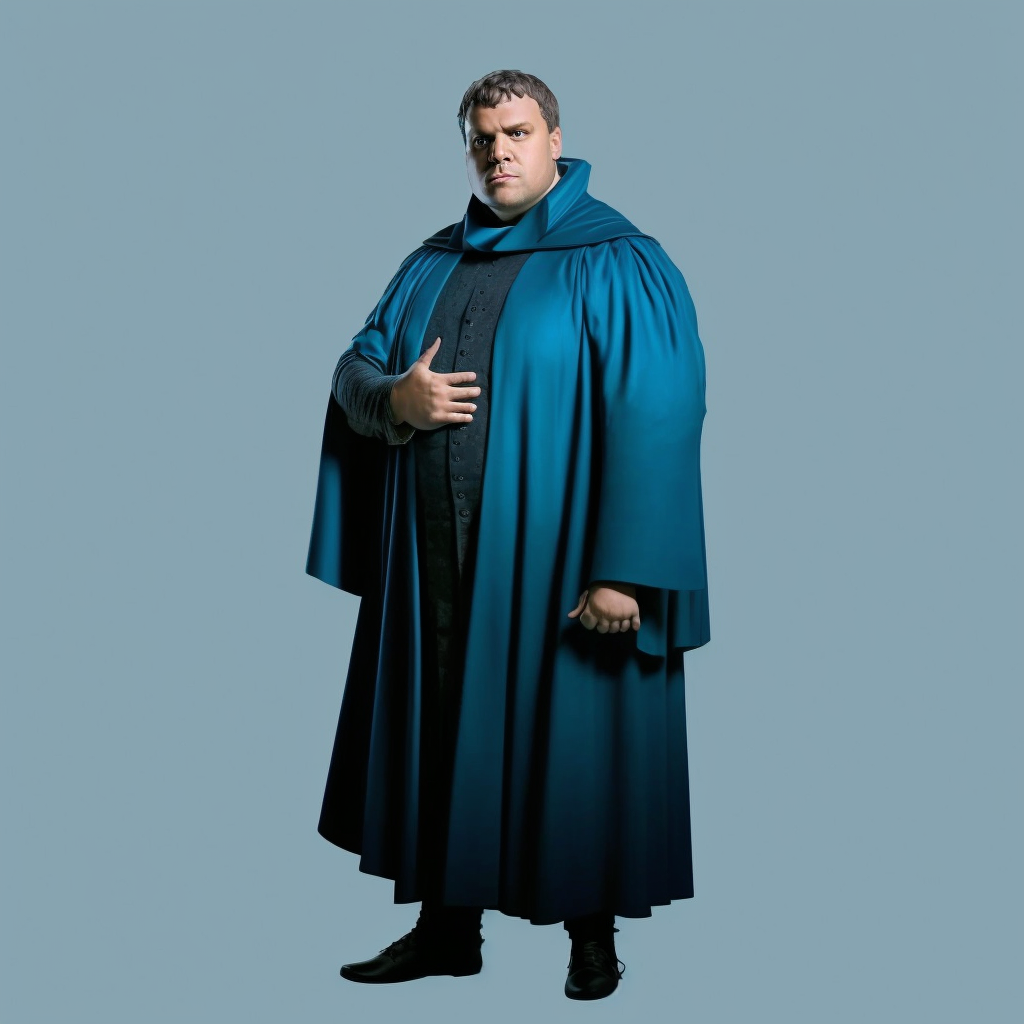
\includegraphics[width=6.405cm\linewidth]{BilderFuerBA/ersteMalPIFuHD}
		\caption{Midjourney: Erstes Testbild für PIFuHD}
		\label{erstemalpifuhd}
	\end{minipage}
	\hfill
	\begin{minipage}[t]{0.45\linewidth}
		\centering
		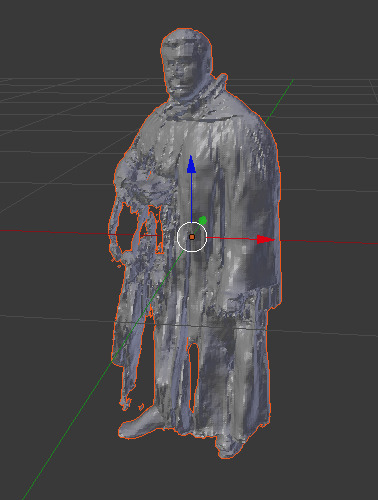
\includegraphics[width=6.405cm\linewidth]{BilderFuerBA/ErsteMalPIFuHDblender}
		\caption{Blender: Erstes 3D-Modell von PIFuHD}
		\label{erstemalpifuhdblender}
	\end{minipage}
\end{figure}
Dieser Test hat mir gezeigt, das es möglich ist, durch MIdjourney generierte Bilder für
\section{weis nicht alles}
Chat GPT ist sehr gut darin unsere Menschliche Sprache zu interpretieren und darauf zu Reagieren. Diesen Vorteil, den ChatGPT besitzt möchte ich an dieser Stelle mir zu nutzen machen, um mit Midjourney natürlicher zu Komunizieren.
Mein Erste Gedanke und Ansatz in der Richtung war es, das ChatGPT eine Art Dolmecer zwischen mir als Anwender und Midjourney steht.
Midjourney-Prompts sind weniger in Natürlicher Sprache verfasst, sonder eher mehr in Stichworten strukturiert.
Meine erster Gedanke hat sich an dieser Stelle als falsch erwiesen. Die Lösung dieses Problems war es durch einen einfachen Prompt, ChatGPT eine Midjourneyformel beizubringen, was gut funktioniert hat.
Das Problem was anschließend daraus entstand, ist Das ChatGPT immernoch nicht gute Midjourney-Promts erzeugt.
Als ich für dieses Problem keine Lösung entwickeln konnte, und auch keinen weiteren Lösungsansatz gefunden habe. blieb mir nur noch die Möglichkeit meine Midjourney-Prompts selber zu schreiben und an den gewünschten stellen etwas zu verändern was mich näher zu meinem Ziel bringt.
Abbildung \ref{ChatGPT_erster_Versuch_Midjourney_Promt} zeigt das ich gerne
\section{konsistenz}
Ein Problem möchte ich Gerne mit dem Begriff Konsistenz beschreiben.
KI-Systeme verändern sich und Trainieren sich auch selbst, das bedeutet, das ein Prompt heute nicht das gleiche Ergebnis bring wie in einem Jahr.
Das bedeutet, das neben der Einarbeitung in KI-Systeme auch eine
\begin{figure}
	\centering
	\begin{minipage}[t]{0.45\linewidth}
	\centering
	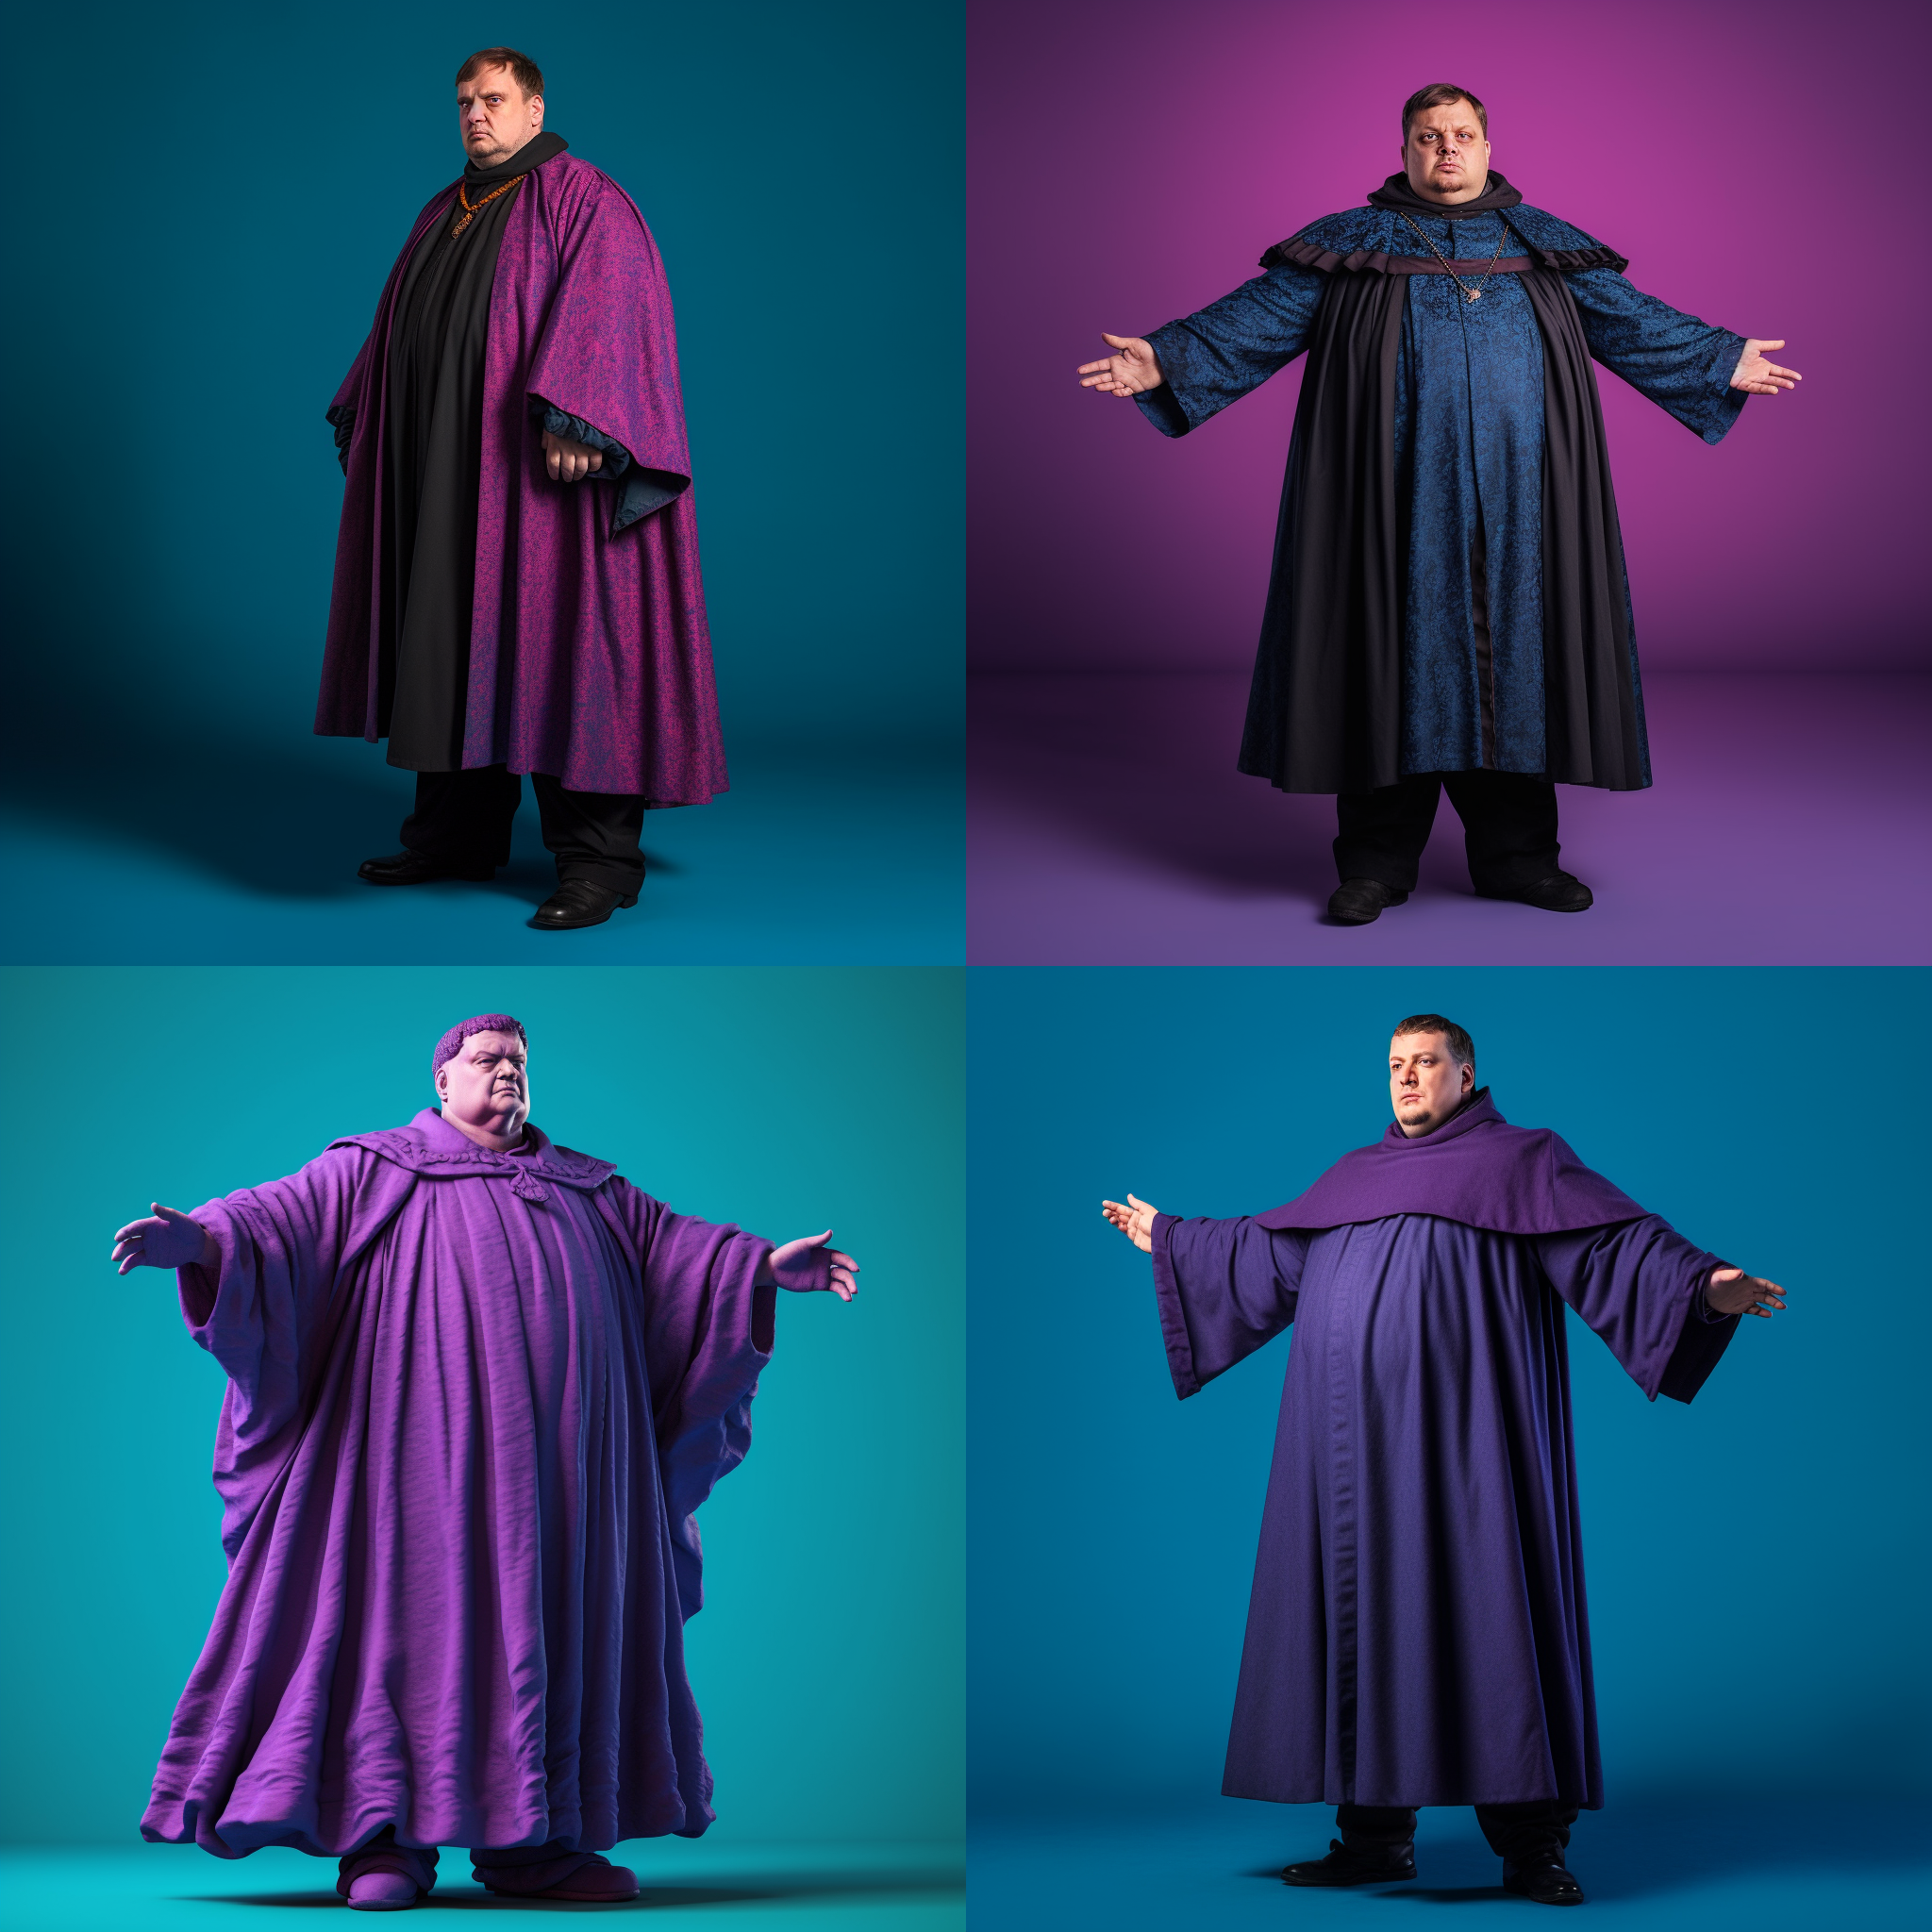
\includegraphics[width=6.405cm\linewidth]{BilderFuerBA/Sonstiges/mlAltSelberSeed}
	
	\end{minipage}
	\hfill
	\begin{minipage}[t]{0.45\linewidth}
	\centering
	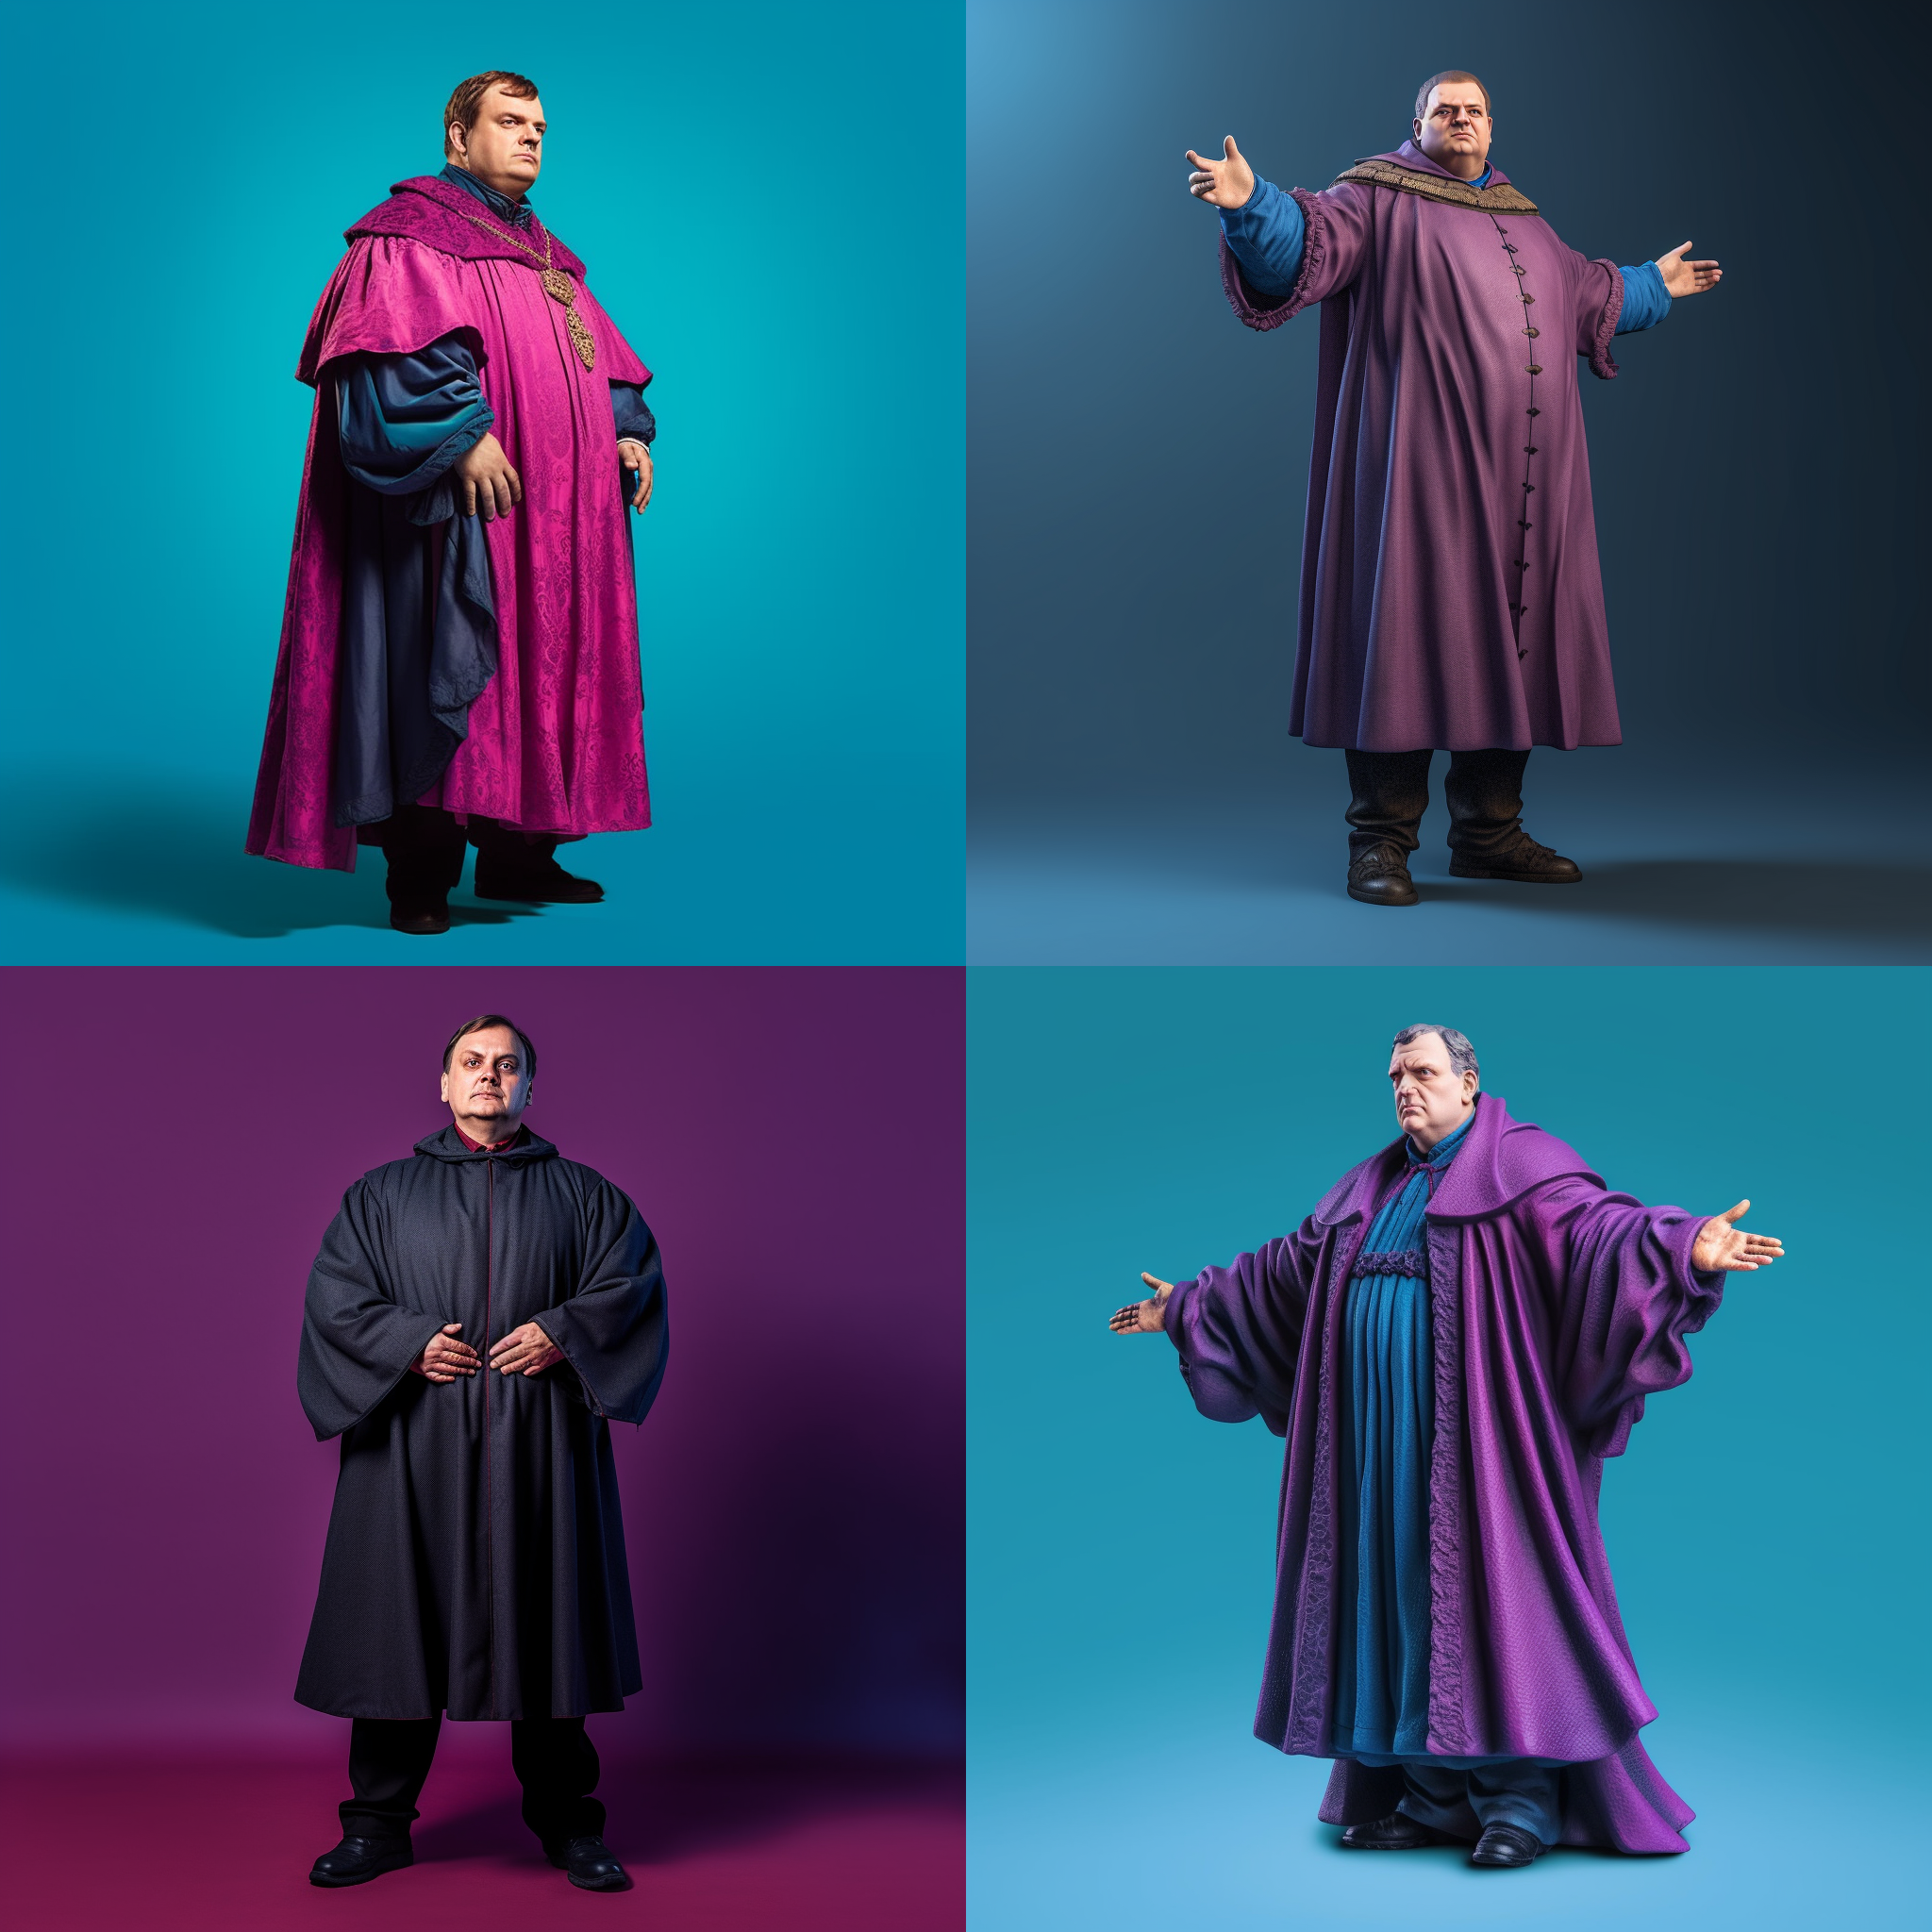
\includegraphics[width=6.405cm\linewidth]{BilderFuerBA/Sonstiges/mlNeuSelberSeed}
	\end{minipage}
	\caption{Midjourney: Vergleich Juni 2023 und Oktober 2023 mit Midj}
	\label{fig:mlaltselberseed}
\end{figure}

\section{rechtliche fragen}
darf ich die bilder benutzen oder nicht... jrmartin klagt gegenüber openAI, midjourney klaurt bilder von großen künstler usw... ein rechliche hochsee was sicher eine eigene ba geben kann
\section{KI-Systeme die ich benutzt habe, aber nicht in das Prototyp beitragen}
irgendwas mit monster mash
\section{T-Pose
\section{oft nur grundgerüst}
das modell von pifuhd muss weiter verarbeitet werden, was kompetenzen erfordert

\chapter{Vorteile }
\section{Zeitersparnis}
100 Texturen innerhalb eines tages, konzeptsuche und ideensuche sowei brainstormen gehen schnell
\section{verbinden von KI-Systemen}
\section{Gute und Günstige Ergebnisse}
viele sachen kostenlos undsehr gute qualität, wie zum beispiel sound datein

